% Preamble
%%%%%%%%%%%%%%%%%%%%%%%%%%%%%%%%%%%%%%%%%%%%%%%%%%%%%%%%%%%%
\documentclass[12pt,letter]{article}
%Layout/Spacing
\documentclass[10pt,letter]{article}
\usepackage[margin=1cm]{geometry} %sets margins
\usepackage[compact]{titlesec}%sets margins
\usepackage{setspace} %singles spacing
\usepackage{fullpage} %use entire page
\usepackage{amsmath} %for math command
%Graphics
\usepackage{graphicx} %for inserting pics
\usepackage{pgfplots} %for simple plots
\usepackage[section]{placeins} %for FloatBarrier
\usepackage[linguistics]{forest} %for forests
\usepackage{tikz}% for flow chart
\usetikzlibrary{shapes,arrows,positioning,fit,quotes,shapes.misc}% for flow chart
%Tables
\usepackage{tabularx}
\usepackage{multirow}
\usepackage{array}
%References
\usepackage[natbib=true,style=authoryear,backend=biber,useprefix=true]{biblatex}
\addbibresource{refs.bib}

% Math Stuff 
%%%%%%%%%%%%%%%%%%%%%%%%%%%%%%%%%%%%%%%%%%%%%%%%%%%%%%%%%%%%
% Piecewise function
\[\mu(g,e) = \begin{dcases}
           \mu_R & r \in g, e \neq E_a \\
    \sqrt{\mu_R} & r \in g, e = E_a \\
           \mu_r & R \in g, e \neq E_a \\
    \sqrt{\mu_r} & R \in g, e = E_a \\
          \end{dcases}\]

% Labelled matrix
%%%%%%%%%%%%%%%%%%%%%%%%%%%%%%%%%%%%%%%%%%%%%%%%%%%%%%%%%%%%
$$\begin{blockarray}{c|cccccccc}
& D& E& F& I& L& Q& V& W \\
\hline
\begin{block}{c|cccccccc}
%  D E F I L Q V W
D&0&1&0&0&0&0&0&0\\
E&1&6&0&0&0&1&0&0\\
F&0&0&4&0&0&0&0&1\\
I&0&0&0&0&0&0&1&0\\
L&0&0&0&0&0&0&1&0\\
Q&0&1&0&0&0&0&0&0\\
V&0&0&0&1&1&0&6&0\\
W&0&0&1&0&0&0&0&4\\
\end{block}
\end{blockarray}$$

% Figures 
%%%%%%%%%%%%%%%%%%%%%%%%%%%%%%%%%%%%%%%%%%%%%%%%%%%%%%%%%%%%
%% Text around figures
This is above the image
\begin{center}
\FloatBarrier
\begin{figure}[htb!]
    \makebox[\textwidth][c]{\includegraphics[width=\linewidth]{example.png}}
    \caption{This is a caption}
    \ref{fig}
\end{figure}
\FloatBarrier
\end{center}
This is bellow the image and references figure \label{fig}
%% subfigures
\FloatBarrier
\begin{figure}[htb!]
    \centering
    \begin{subfigure}[t]{0.45\textwidth}
        \centering
        \makebox[\textwidth][c]{\includegraphics[width=\linewidth]{./figures/Singular_Antibiotic.png}}
        \caption{Single Antibiotic Event, event starts at green dotted line and ends at red dotted line.l=50}
    \end{subfigure}
    \begin{subfigure}[t]{0.45\textwidth}
        \centering
        \makebox[\textwidth][c]{\includegraphics[width=\linewidth]{./figures/Singular_Phage.png}}
        \caption{Single Phage Event, event starts at green dotted line and ends at red dotted line. l=50}
    \end{subfigure}
    \caption{Single event simulations.}
\end{figure}
\FloatBarrier

% Newtwork diagrams
%%%%%%%%%%%%%%%%%%%%%%%%%%%%%%%%%%%%%%%%%%%%%%%%%%%%%%%%%%%%
\usepackage{tikz-network}
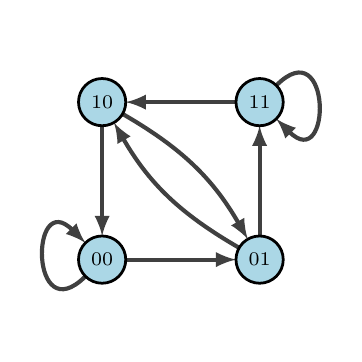
\begin{tikzpicture}
    \Vertex[x=0,y=0,label=00]{A}
    \Vertex[x=2,y=0,label=01]{B}
    \Vertex[x=0,y=2,label=10]{C}
    \Vertex[x=2,y=2,label=11]{D}
    \Edge[Direct,loopposition=-180](A)(A)
    \Edge[Direct](D)(D)
    \Edge[Direct](A)(B)
    \Edge[Direct](C)(A)
    \Edge[Direct,bend=15](C)(B)
    \Edge[Direct,bend=15](B)(C)
    \Edge[Direct](B)(D)
    \Edge[Direct](D)(C)
\end{tikzpicture}

% Simple Plot
%%%%%%%%%%%%%%%%%%%%%%%%%%%%%%%%%%%%%%%%%%%%%%%%%%%%%%%%%%%%
\usepackage{pgfplots} %for simple plots
\begin{documents}
%Tikz pgfplots
\begin{center}
\begin{tikzpicture}
    \begin{axis}[ xlabel = $N_e$, ylabel = $\mu$]
        \addplot[color=blue]{-x};
    \end{axis}
\end{tikzpicture}
\hspace{0.5in}
\begin{tikzpicture}
    \begin{axis}[ xlabel = $N_e$, ylabel = Generation Time]
        \addplot[color=blue]{-x};
    \end{axis}
\end{tikzpicture}
\begin{center}
    \begin{tikzpicture}
        \begin{axis}[xlabel = Generation Time,ylabel = $\mu$]
            \addplot[color=red]{x};
        \end{axis}
    \end{tikzpicture}
\end{center}

% Pseudocode
%%%%%%%%%%%%%%%%%%%%%%%%%%%%%%%%%%%%%%%%%%%%%%%%%%%%%%%%%%%%
\usepackage{algorithm}
\usepackage{algorithmic}

Pseudocode for this algorithm is as follows
\begin{algorithm}
\caption{Find $r(e) \forall\; e \in T$}
    \begin{algorithmic}
        \STATE $r_e \leftarrow \{t_i:t_i\} \;\forall\; t \in E(T)$ // associative array for all edges in $T$
        \STATE $E' \leftarrow sort(E(G) - E(T))$ // sorted (ascending) list of edges of $G$ excluding edges in $T$
        \FOR {$t \in E(T)$}
            \STATE $T' \leftarrow T - t$ // $T'$ has 2 connected components $T_!, T_2$
            \FOR {$e =\{v,w\} \in E'$}
                \STATE // if edge $e$ connects both components of $T'$
                \IF{$v \in T_1 \land w \in T_2$}
                    \STATE $r_e[t] \leftarrow e$
                \ENDIF
            \ENDFOR
        \ENDFOR
        \RETURN $r_e$ //associative array where keys are edges in $T$ and values are replacement edges from $G$
    \end{algorithmic}
\end{algorithm}

% Tree Diagram
%%%%%%%%%%%%%%%%%%%%%%%%%%%%%%%%%%%%%%%%%%%%%%%%%%%%%%%%%%%%
\usepackage[linguistics]{forest} %for forests
\begin{center}
    \scalebox{2.0}{
    \begin{forest}
        for tree={
            if n children=0{
                font=\itshape,
                tier=terminal, %lines up all tips together
            }{},
        }
        [
         [
          [Old World Monkeys
           [Apes
            [
             [Human]
             [
              [Chimp]
              [Bonobo]
             ]
            ]
            [Orangutan]
           ]
           [Macaque]
          ]
          [Prosiminans
           [Howler]
          ]
         ]
         [Tarsiers
          [Lemur]
         ]
        ]
    \end{forest}}
\end{center}

